Let us now go back to the issue of imputing missing data when there is a separation between the Practitioner and the Analyst, that is, when it is necessary to impute new incoming data without having access to the historical data.

As described Chapter \ref{imputation}, a number of methods exist to impute missing data. However, they have been designed with parameter estimation in mind: in that case, there is just one dataset that needs to be imputed. The issue, as we show in this chapter, is that current implementations of these methods may not be suitable when we need to use the same model to impute two separate datasets.

This is not only problematic for our particular problem. As we remind in Section \ref{ERM}, it is standard practice when working on prediction to resort to CV, that is to hold out part of the data and use it to validate the model. Section \ref{ERM.imp} shows how this clashes with current implementation of imputation methods. In section \ref{ERM.solutions}, we investigate possible ways to address this issue and compare them empirically.

%On the other hand, there is almost no research on these methods when applied to prediction. Even recent manuals for machine learning \cite{ML_missdata} generally make only a quick mention of missing data, and in practice it is extremely rare for anything else than imputation by the mean to be used. \emph{Scikit-learn} \cite{scikit-learn}, by far the most-used machine learning package, only proposes imputation by the mean as of now. 

%A few research papers \cite{prediction_imputation1} \cite{prediction_imputation2} try to assess the performance of more recent imputation methods when used in a predictive context. However, they do not propose any framework or theory on this endeavour. They take it for granted that they can impute the whole dataset before performing the subsequent analysis. However, when performing prediction there is one significant difference with statistical inference, which we describe further in this chapter: the data is split into one dataset to learn the model, and another one to validate its performance. This raises many questions that we discuss here and in Chapter \ref{linreg}. 

%After laying out the general framework of Empirical Risk Minimization \cite{ERM}, which is the general paradigm used for prediction, we adapt it to fit the context of missing data. We notice that current implementations of modern imputation methods are incompatible with this framework, and try to devise solutions for this issue.
	\section{Empirical risk minimization and cross-validation}
	\label{ERM}
Let us start by ignoring the issue of missing data and assume that the data is complete. That is, we place ourselves in the same situation as described in \ref{framework} but there is no need for an Imputer, and the Analyst directly receives the data $X$.
	
As stated in Chapter \ref{data}, our end goal is to make good predictions in the real world by learning on historical data. Of course, by definition we do not have access to any future data right now, but we still need to choose a prediction and imputation model, and estimate how it will perform when we use it on the field. 

To learn and evaluate the model, we go through two steps: Empirical risk minimization (ERM) and cross-validation (CV). We describe them below
		\subsection{Empirical risk minimization}
Let us denote the $X$ a $n \times p$ matrix of covariates and $y$ a response vector of size $n$, where our goal is to predict the response $y_{new}$ from some future data $X_{new}$, assuming that $(X_{new}, y_{new}$ follow the same distribution as $X,y$. 

We choose a class of functions $f(\cdot, \beta), \beta \in B$. We want to choose a parameter $\hat{\beta}$ which we can use to predict $\hat{y}_{new} = f(X_{new}, \hat{\beta})$.  The quality of a prediction is evaluated by some loss $L(y_{new},\hat{y}_{new})$. Since we do not have access to $X_{new}$, our goal is to minimize the risk: $R(\beta) = \mathbb{E}_{X_{new},y_{new}}(L(y_{new}, f(X_{new}, \beta)))$.

However, we do not know the true distribution of those values. This is why we resort to ERM \cite{ERM}: we define the empirical risk
$$ R_{\text{emp}}(\beta) = \frac{1}{n} \sum\limits_{i=1}^n L(y_i, f(X_i, \beta))$$
that is, the average value of the loss when predicting the known $y$  from $X$ with $\beta$.

We then select $\hat{\beta} = \argmin_{\beta} R_{\text{emp}}(\beta)$ as our ERM estimator for $\beta$. However, this is not enough. Once we have chosen $\hat{\beta}$, we need to have an estimate of how well this estimate will perform on new data.

 This is important because this is what we will take into account if we need to compare multiple choices for $f$. But the empirical risk gives us no measure of how well our model generalizes, only of how closely it can fit known data. In particular, if the class $f$ is very broad, one may find a $\beta$ that exactly interpolates the values of $y$ but does not generalize at all (an issue known as overfitting \cite{hawkins2004overfitting}

To address the issue of model selection, we need to resort to CV as descried below.

		\subsection{Cross-validation}
CV, consists in dividing the available data in two datasets: first we choose $n_A < n$ entries in the dataset that will be used in ERM to learn $\hat{\beta}$: this is the training dataset $X_A$ and response $y_A$. We denote $I_A = (i_1, \ldots, i_{n_A})$ the set of indices chosen for the training data.

The rest of the observations are noted $X_V$ and $y_V$ and called the validation dataset. They are used as a substitute for $X_{new},y_{new}$

Once this is done, the Analyst performs ERM as before, using only the training data. The obtained parameter $\hat{\beta}$ can then be evaluated with the validation error:

$$ R_{V}(\hat{\beta}) = \frac{1}{n_V} \sum\limits_{i=1, i \notin I_A}^n L(y_i, f(X_i, \hat{\beta}))$$

It is this value that we can compare to choose the model class $f$. Once the Analyst has decided on a choice of $f$ and $\hat{\beta}$ using ERM and CV, she can send $f(\cdot, \hat{\beta})$ over to the Practitioner so that she can proceed to prediction on new data using $\hat{y_{new}} = f(X_{new}, \hat{\beta})$.

	\section{ERM with missing data: the problem of current methodologies}
	\label{ERM.imp}
We now place ourselves in the same context as before, except some values are missing from $X$, both in the training and the validation data. This means that we are back to a case where there is an Imputer in addition to the Analyst.
		\subsection{Imputation seen as an ERM}
Remember that the purpose of this work is to impute the data independently of the model used afterwards for prediction. This means that we cannot perform ERM exactly as before and use any function we like to go from $X$ (which has missing data) to $\hat{y}$. The prediction is the composition of two steps.
			\paragraph{Imputation step}
First we choose an imputation model $X^{\text{complete}} = g(X, \alpha)$ where $X^{\text{complete}}$ is the completed dataset and $\alpha$ some parameter. This is similar to the previously described ERM, except we do not know the true data (while we had $y$ to compare to $\hat{y}$, we do not know the true full dataset $\tilde{X}$). Thus, we choose $\hat{\alpha}$ to minimize some unsupervised empirical risk
$$R'_{emp}(\alpha)=L'(g(X, \alpha), \alpha)$$
Sometimes the loss $L'$ is related to the likelihood of the completed data according to some distribution\cite{ref_amelia} (though it is not always the case \cite{stekhoven2015missforest}). Once this is done, we obtain a completed dataset $\hat{X}$.

			\paragraph{Prediction step}
With imputation done, we can proceed as before to choose a parameter $\hat{\beta}$ that minimizes the empirical risk when using the completed data:
	$$ R_{\text{emp}}(\beta, \hat{X}) = \frac{1}{n} \sum\limits_{i=1}^n L(y_i, f(\hat{X}_i, \beta))$$
	
Putting it all together, we can define 
$$ h(X, (\alpha, \beta)) = f(X^{imp}, \beta) = f( g(X, \alpha), \beta) $$
the combined model that takes the observed data as input and outputs a predicted $y$. Formally, the two successive steps yield:
\begin{align*}
\hat{\alpha} &= \argmin_{\alpha} L'(g(X,\alpha) \\
\hat{\beta} &= \argmin_{\beta} R_{\text{emp}}(\beta,f(X,\hat{\alpha})) \\
\hat{y} &= h(X, (\hat{\alpha}, \hat{\beta}))
\end{align*}

We choose to use this notation to illustrate our point that imputation is an integral part of the ERM, not a separate, preliminary process. In particular, it means that its parameters must be subjected to CV just like those of the prediction. That is, only $X_A$ and $y_A$ are used to estimate $(\hat{\alpha}, \hat{\beta})$ as shown above, while $X_V$ and $y_V$ are held out. Then, we can compute a prediction $\hat{y}_V = h(X_V, (\hat{\beta}, \hat{\alpha}))$ and we compute $L(y_V, \hat{y}_V)$ to evaluate the choice of model.

This implies that just like $\beta$, the imputation parameter $\alpha$ should be estimated only on the training data and then used on the validation data. As we will see, this raises an issue with the way current imputation methods are implemented.

		\subsection{Unsuitability of current methods}
Implementations of imputation methods have one thing in common: they are used through a single function which takes a dataset with missing values as an input and returns the dataset completed by the method of choice, \emph{without giving the user any access to the imputation model itself}. \cite{stekhoven2015missforest} \cite{josse2016missmda}\cite{MICE_founding}\cite{ref_amelia}

This is a problem because of how CV is supposed to be performed. Supposedly, one would estimate $(\hat{\alpha}_A, \hat{\beta}_A)$ through ERM, and then make a prediction on the validation set as $h(X_V,(\hat{\beta}_{X_A},\hat{\alpha}_{X_A}))$. But here, all we have access to is a black-box function $g': X \mapsto g(X, \hat{\alpha}_X)$ where $\hat{\alpha}_X$ is the optimised parameter for the argument $X$. This means that one cannot choose what parameters are used to impute the input to function $g'$: a new parameter will be estimated at every call of the function. But in that case, it is impossible to use the same $\alpha$ for the training dataset and for the validation data --- or for new data.
	
This issue has started to arise in the machine learning community in the past few years \cite{thread_newdata1}\cite{thread_newdata2}\cite{thread_newdata3}, but for now no implementation exists that separates the parameter estimation and the imputation itself (except for the very basic imputation by the mean \cite{mean_imputation}). Below, we investigate the alternatives available to perform imputation with held out data.

	\section{Possible solutions}
	\label{ERM.solutions}
	
If we were to follow exactly the principles of CV, we would proceed as follows: 
\begin{algorithm}[H]
	\caption{Identical imputation}
	\hspace*{\algorithmicindent} \textbf{Input:} $X$, $y$, $I_A={i, X_i \in X_A}$  \\
 	\hspace*{\algorithmicindent} \textbf{Output:} $\hat{y}_V$
	\begin{algorithmic}[1]
		\State \textbf{Parameter estimation:}
		\Indstate $\hat{\alpha}_A \leftarrow \argmin_{\alpha} L'(g(X_A,\alpha)$
		\Indstate $\hat{X}_A \leftarrow g(X_A, \hat{\alpha}_A)$
		\Indstate $\hat{\beta}_A \leftarrow \argmin_{\beta} R_{\text{emp}}(\beta,\hat{X}_A)$
		\State \textbf{Prediction:}
		\Indstate $\hat{X}_V \leftarrow g(X_V, \hat{\alpha}_A)$ \Comment \emph{Uses the same $\alpha$ as for the training set}
		\Indstate $\hat{y}_V \leftarrow f(\hat{X_V}, \hat{\beta}_A)$
	\end{algorithmic}
\end{algorithm}

But this is not possible using a black-box function because we need to recover $\hat{\alpha}_A$ and reuse it with $X_V$.

		\subsection{Alternatives using current implementations}
			\subsubsection{Methods}

Suppose we only have access to the back-box $g'$ described above. Then there are two main ways of performing the imputation.

\paragraph{Grouped imputation} 

Impute all the data at once before performing the CV split:
\begin{algorithm}[H]
	\caption{Grouped imputation}
	\hspace*{\algorithmicindent} \textbf{Input:} $X$, $y$, $I_A={i, X_i \in X_A}$  \\
 	\hspace*{\algorithmicindent} \textbf{Output:} $\hat{y}_V$
	\begin{algorithmic}[1]
		\State \textbf{Imputation:}
		\Indstate $\hat{X} \leftarrow g'(X) = g(X, \hat{\alpha}_X)$ 
		\Indstate $(\hat{X}_A, \hat{X}_V) \leftarrow \hat{X}$ \Comment \emph{Split the data after imputation}
		\State \textbf{Estimation of the prediction parameter}
		\Indstate $\hat{\beta}_A \leftarrow \argmin_{\beta} R_{\text{emp}}(\beta,\hat{X}_A)$ \Comment \emph{Note that $\hat{X}_A = g(X_A, \hat{\alpha}_X)$}
		\State \textbf{Prediction:}
		\Indstate $\hat{y}_V \leftarrow f(\hat{X_V}, \hat{\beta}_A) = f(g(X_V, \hat{\alpha}_X)$
	\end{algorithmic}
\end{algorithm}

Here, both datasets are indeed imputed with the same parameter $\alpha_X$ but this means that the validation data is used to choose that parameter which then serves to impute the training data. This is contrary to the principles of CV, we are 'cheating' in some way.

\paragraph{Separate imputation}
Divide the data first, then impute each dataset separately:
\begin{algorithm}[H]
	\caption{Separate imputation}
	\hspace*{\algorithmicindent} \textbf{Input:} $X$, $y$, $I_A={i, X_i \in X_A}$  \\
 	\hspace*{\algorithmicindent} \textbf{Output:} $\hat{y}_V$
	\begin{algorithmic}[1]
		\State \textbf{Training parameter estimation:}
		\Indstate $\hat{X}_A \leftarrow g'(X_A) = g(X_A, \hat{\alpha}_A)$
		\Indstate $\hat{\beta}_A \leftarrow \argmin_{\beta} R_{\text{emp}}(\beta,\hat{X}_A)$
		\State \textbf{Imputation of $X_V$:}
		\Indstate $\hat{X}_V \leftarrow g'(X_V) = g(X_V, \hat{\alpha}_V)$ \Comment \emph{Imputation made independently of that of $X_A$}
		\State \textbf{Prediction:}
		\Indstate $\hat{y}_V \leftarrow f(\hat{X_V}, \hat{\beta}_A)$
	\end{algorithmic}
\end{algorithm}

Contrarily to grouped imputation, we are not cheating. However, we are using parameter $\hat{\alpha}_V$ to impute $X_V$, while we learned $\hat{\beta}_A$ on $\hat{X}_A$ which was imputed with $\hat{\alpha}_A$. That is, we are optimising $h(\cdot,(\hat{\alpha}_A, \hat{\beta}_A$ and predicting with  $h(\cdot,(\hat{\alpha}_V, \hat{\beta}_A$.

$\hat{\alpha}_V$, $\hat{\alpha}_A$ and $\hat{\alpha}_X$ are asymptotically the same for large $n$ --- since $X_A$, $X_V$ and $X$ have the same distribution ---, so all three methods should be identical for large $n$. But for smaller $n$, harmful effects may be present --- overoptimistic validation due to 'cheating' for the grouped imputation, high error due to the difference in parameters for separate imputation.

%\paragraph{Line by line imputation}
%The last option we mention here is to first impute the training data on its own. Then for every line of the validation data we impute it by stacking it with the imputed training data and imputing the whole dataset. Since it is just one line, we can safely assume that the imputation parameters will be those of the training data. The main issue with this method is that is the validation data is rather large, this will be computationally infeasible.

			\subsubsection{Need for a new implementation}
We want to understand if the alternatives proposed here are good enough to be used if Identical imputation in infeasible (e.g. we want to evaluate a new imputation method that only implements a black box). To do that, we need to be able to compare these with the correct method. That means that for at least one imputation method we need to build an implementation that allows us to separate the estimation and the imputation. That way we will be able to compare its performance with the other alternatives we propose.

Moreover, in addition to this theoretical pursuit, we need this because of what we are trying to achieve with Traumabase: the end goal is to make a recommendation system that can produce a prediction for \emph{a single new patient} arriving to the hospital, without needing to have access to the whole Traumabase data. Without access to the initial training data, this means that only a fully parametric approach can be taken in this particular case (separate imputation is impossible on just one line of data, and grouped imputation requires access to the full data).

Below, we design a very simple imputation method for those purposes.

		\subsection{Multivariate normal conditional expectation}
The principle of this imputation is inspired from R package \emph{Amelia} \cite{ref_amelia}, and a large part of the code is from the \emph{norm} package \cite{pkg_norm}. The idea is to model both $X_A$ and $X_V$ as normally distributed $\mathcal{N}(\mu, \Sigma)$ with unknown parameters. This will allow us to impute the missing data conditionally on the observed data.

\paragraph{Parameter estimation}
It is possible to approximate maximum-likelihood estimators for $\mu$ and $\sigma$ with an iterative procedure, using the EM (expectation-maximisation) algorithm \cite{EM} \cite{em_normal_fit}. The algorithm is as follows:
\begin{algorithm}[H]
	\caption{Normal parameter estimation with EM}
	\hspace*{\algorithmicindent} \textbf{Input:} $X$  \\
 	\hspace*{\algorithmicindent} \textbf{Output:} $\hat{\mu}, \hat{\Sigma}$
	\begin{algorithmic}[1]
		\State $X^{(0)} \leftarrow X$ where missing values are replaced using the observed mean of $X$ (mean imputation)
		\State $t \leftarrow 0$
		\While {not converged}
			\State $(\mu^{(t)}, \Sigma^{(t)}) \leftarrow$  sample mean and covariance matrix of $X^{(t)}$ \Comment \emph{i.e. maximum likelihood estimates on the completed data}
			\State $X^{(t+1)} \leftarrow  \mathbb{E}_{X^{\text{miss}}}(X \vert X^{\text{obs}} ; \mu^{(t)}, \Sigma^{(t)})$ \Comment \emph{Missing values are replaced by their expected value under the new parameters}
			\State $t \leftarrow t+1$
		\EndWhile
		\State $\hat{\mu}, \hat{\Sigma}$ = $\mu^{(t)}, \Sigma^{(t)}$
	\end{algorithmic}
\end{algorithm}

The conditional expectations are easily derived using the Schur complement \cite{norm_schur}. For this step, we use a slightly modified version of the code from the \emph{norm} package. In all that comes next, unless specified otherwise this imputation method is the one we use, with identical imputation.

\paragraph{Imputation}
Once we have the parameters, it is very straightforward to get an imputation of the missing data. Just as during the EM procedure, we impute using the conditional expectation of the dataset conditioned on the observed values: 
$$\hat{X} = \mathbb{E}_{X^{\text{miss}}}(X \vert X^{\text{obs}} ; \hat{\mu}, \hat{\Sigma})$$

We implemented this step as well to get a complete imputation procedure divided in two functions that implement the estimation and imputation steps separately. The code is available in package \todo{make package and insert reference}

		\subsection{Comparison on simulated data}
Now that we have an implementation that separates estimation and imputation, we use it to compare the three imputation procedures on simulated data (cf Appendix \ref{simulation}, with $\rho=0.5, p=4, \sigma=1$) and the abalone data (cf Appendix \ref{abalone}) with various sample sizes and adding 30\% missing data MCAR.  The results are in Figure \ref{fig.grouped_separate}.

\begin{figure}[h]
  \centering
  \subbottom[Results for simulated data]{%
    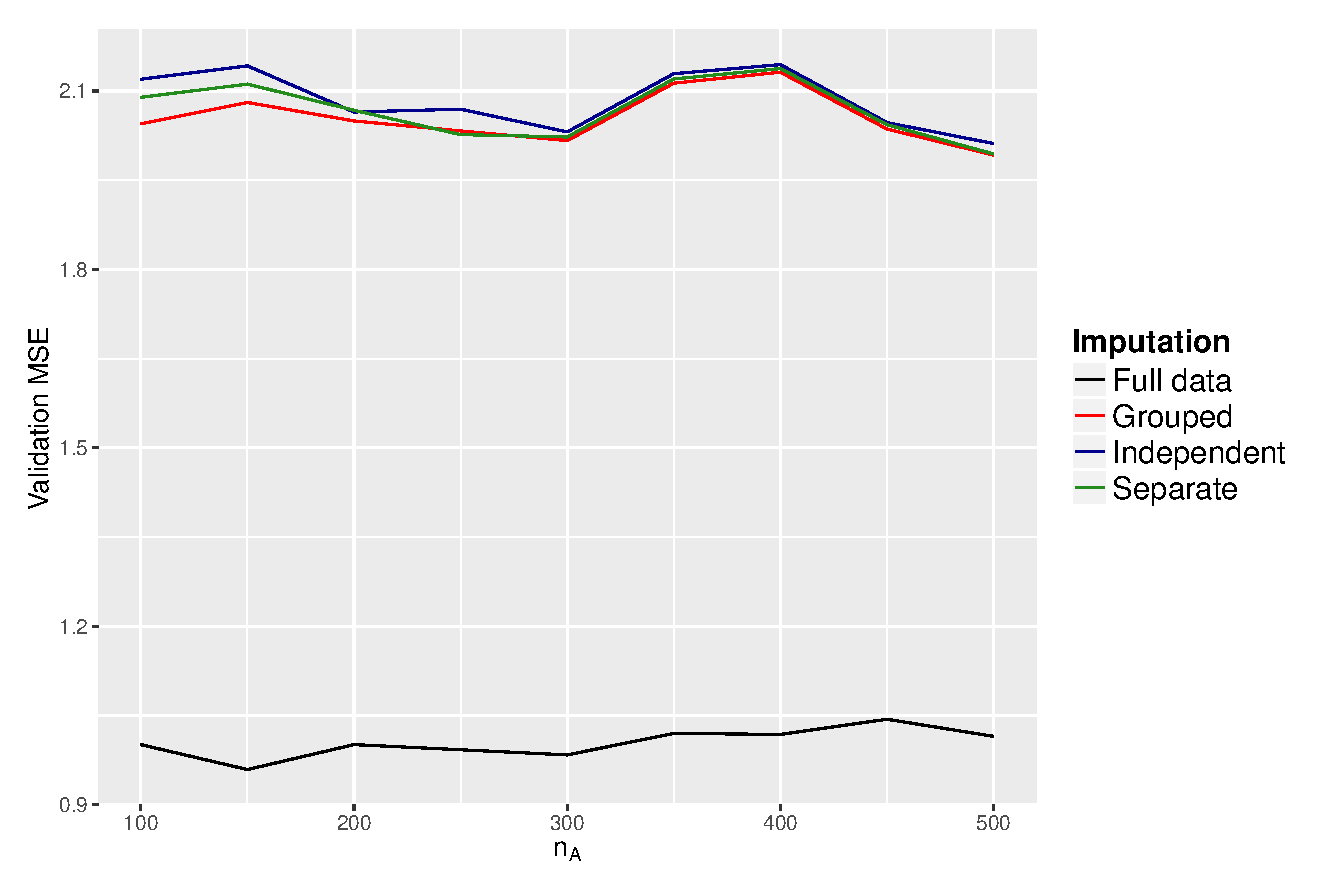
\includegraphics[scale=0.5]{Resources/grouped_separate_sim}}\\
  \subbottom[Results for abalone data]{%
    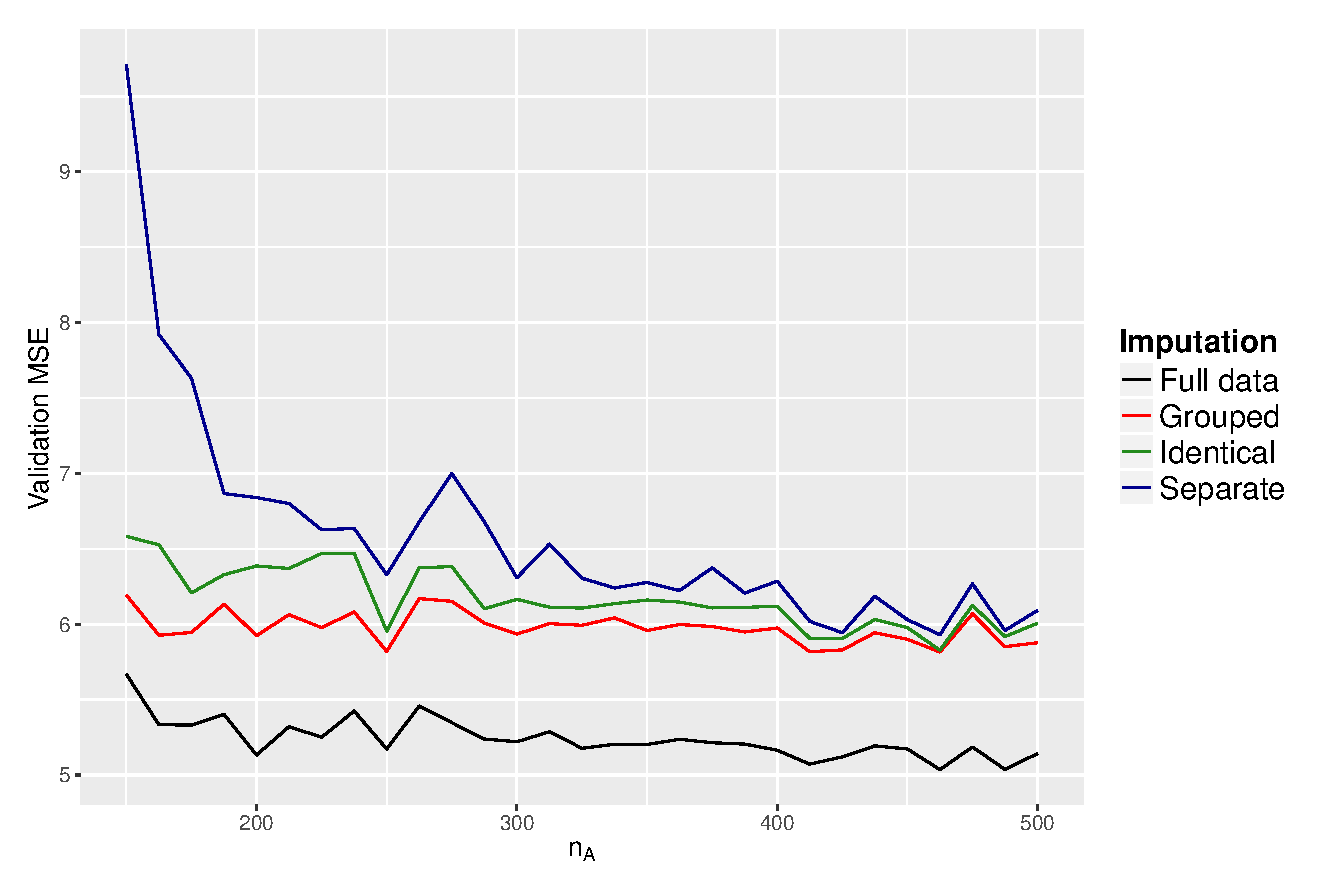
\includegraphics[scale=0.5]{Resources/grouped_separate_aba}}
  \caption{Comparison of imputation methodologies (averaged over 100 runs)}
  	\label{fig.grouped_separate}  
\end{figure}
	
We see that indeed grouped imputation seems to always have lower error than identical imputation, while separate imputation has higher error. However, when $n$ is not too small, all three are quite close together. Separate imputation seems to be further off than the other two, and sometimes has very high error. As a result, if no implementation exists for a given method to perform identical imputation, trying it out with grouped imputation would be a good first step to get an idea of how it can perform.

Still, for real applications, imputation must be performed on new data without having the training data at hand, so once an imputation method is chosen, is would be necessary to implement it in a way that allows identical imputation.